\scanpage{16}
\mspage{14}

\margin{\figure{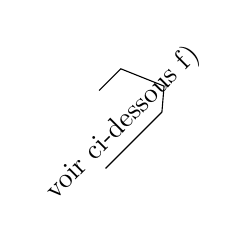
\begin{tikzpicture}[x=0.55cm,y=0.55cm]\draw (0,1.8)--(.5,2.3)--(1.5,1.9)--(1.45,1.3)--(.15,0);\node[rotate=45] at (.55,1.05) {\uline{voir ci-dessous \unsure{f)}}};\end{tikzpicture}}}
\deleted{\unsure{f)}}\inserted{\unsure{g)}} \uline{Faisceautisation} Il y a une définition évidente de complexes de De Rham à p.d. sur $k$ si $k$ est un Anneau comm. d'un topos. On aimerait, p.ex. en comparant un tel complexe à un autre qu. iso. dont les composantes soient flasques (mais y en a-t-il tjrs ?) définir des \unsure{op.\textsuperscript{s}} $Rf_*$ dans des cat. dérivées convenables pour de tels complexes, quand $f:\mathcal X\to\mathcal Y$ est un morphisme de topos \inserted{(\unsure{appropriées au-dessus des deux cat. faisc.}\dots)} Si $k$ est une $\mathbb Q$-Algèbre, le $=$ Pb se rencontre d'ailleurs déjà pour les complexes du type De Rham-Sullivan, et le Pb est ouvert -- et posé par Deligne -- pour $\mathcal X=(\mathrm{Ens})^{\unsure{I}}=\text{topos des ens. cosimpliciaux}$, $\mathcal Y=\text{topos ponctuel}$. Mais sauf erreur (si \unsure{souvenirs} sont exacts) il y a un topo qui marche, pour les espaces \inserted{topologiques} paracompacts\dots

\mspage{15}
